\documentclass{article}
\usepackage[T1]{fontenc}
\usepackage{lmodern}
\usepackage{graphicx}
\usepackage{amsmath,amssymb}
\usepackage[a4paper,margin=2cm]{geometry}
\usepackage[absolute,overlay]{textpos}
\setlength{\TPHorizModule}{1mm}
\setlength{\TPVertModule}{1mm}
\usepackage[indonesian]{babel}
\usepackage{hyperref}
\setlength{\emergencystretch}{2em}
% unit: Halaman 95

\begin{document}

% === Halaman 95 (python/native) ===

Referensi

• Li, F., The art and science of writing hidden messages: Steganography

• Khan, M. M. , Steganography

• Wohlgemuth, S. (2002), IT-Security: Theory and Practice : Steganography and Watermarking, 

University of  Freiburg, Denmakr, 2002.

• Tawalbeh, L. (2006), Watermarking, Information System Security, AABFS-Jordan.

95

% deskripsi: gambar native xref 384
\noindent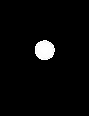
\includegraphics[width=0.85\textwidth]{../../images/python/page_095_img_01.png}

% deskripsi: gambar native xref 386
\noindent
\includegraphics[width=0.85\textwidth]{../../images/python/page_095_img_02.png}

% deskripsi: gambar native xref 388
\noindent
\includegraphics[width=0.85\textwidth]{../../images/python/page_095_img_03.png}

\end{document}
